\documentclass{vgtc}

\usepackage{mathptmx}
\usepackage{graphicx}
\usepackage{times}
\usepackage{epsfig}

\onlineid{0}

\vgtccategory{Research}

\vgtcinsertpkg

\title{SwarmVis: a Tool for Visualizing Swarm Systems}

\author{Don Miner\thanks{e-mail: don1@umbc.edu}\\ %
        \scriptsize University of Maryland, Baltimore County %
\and Niels Kasch\thanks{e-mail:nkasch1@umbc.edu}\\ %
     \scriptsize University of Maryland, Baltimore County %
}

\abstract{In this paper, we provide an overview of SwarmVis, a tool for
visualizing swarm systems. SwarmVis integrates several visualization
techniques to create informative still images and videos of swarm
systems moving through two- and three- dimensional space. SwarmVis
allows swarm researchers to observe characteristics of swarm systems by
visualizing information about such systems. We provide an overview of
the types of information relevant to current swarm research and explain,
in detail, the capabilities of SwarmVis to visualize this information.
Finally, we 
demonstrate how SwarmVis can be used to analyze both the local agent and
global swarm behaviors of multi-agent systems.}

\begin{document}

\firstsection{Introduction}

\maketitle

A swarm system is a collection of autonomous agents that, as a group, exhibit some complex behavior.
Examples of these systems include: ants\cite{couzin2003sol}, schooling fish\cite{parrish2002sof}, migrating geese\cite{reynolds1987}, 
and multi-robot systems\cite{mondada2004sbn}\cite{mclurkin2004srt}.
Visualizing swarm systems (swarms) effectively is a non-trivial task, partially due to the large number of individual agents involved.
The high density and chaotic motions of agents found in typical swarms amplify the complexity of swarm visualization.
Effective swarm visualizations are needed to gain insight into local (agent-level) and global (swarm-level) behavior.
A well-defined set of visualization techniques, in combination with an interactive exploratory tool,
provides the facilities to explore these systems at the depth necessary to completely understand them.


Simple visualization techniques can be used to plot the position of each agent in space.
An example of this technique, illustrating a Reynolds boid flock\cite{reynolds1987}, can be seen in Figure \ref{Intro} (left).
The image only shows the location of individual agents but does not convey important
information such as direction, velocity, and previous positions of the agents.

We have implemented \textit{SwarmVis}, a toolkit for visualizing swarms,
that goes beyond the simple plotting method to increase the
expressiveness of swarm visualizations.
The toolkit aims to provide visualization techniques that allow researchers to interactively
investigate a swarm's interactions, fine-grained movements, and behavior.
SwarmVis' still images and animations convey agent-level information such as velocity and direction, as well as swarm-level information such as
structure, direction and rotation.
Figure \ref{Intro} (right) displays a swarm system with SwarmVis' trails visualization, which displays more information.
In this image, direction is expressed by the history of an agent's past positions.
SwarmVis provides a collection of visualizations, which we will discuss in more detail in the Approach section, including
trails, tracks, velocity coloring, group coloring and animation.

After reviewing the visualization techniques available in SwarmVis, we will use these techniques to analyze, in depth,
the tetrahedron-forming swarm. We show what kinds of information can be inferred from the images created by SwarmVis,
both at the swarm-level and the agent-level. This use case is only an example, which can inspire similar analysis in other domains.


\begin{figure}[ht]
\centering
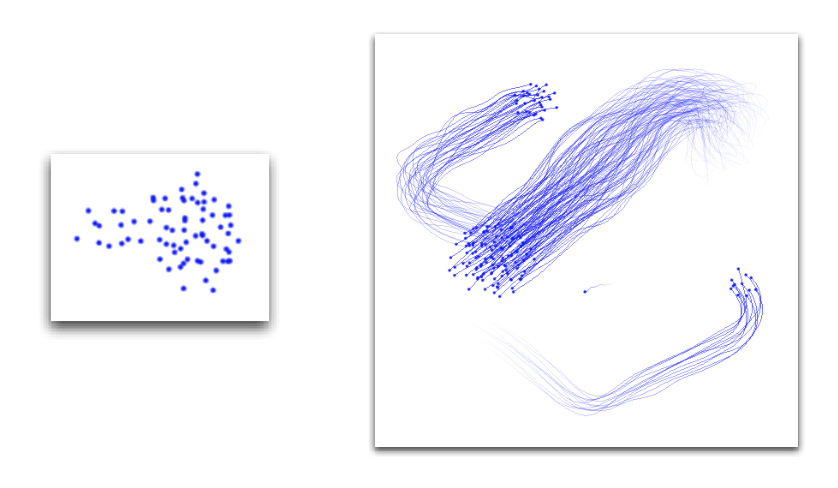
\includegraphics[scale=.55]{images/intro.pdf}
\caption{(Left) A basic visualization of a boid flock with agents are plotted as
points in space. The image only conveys positional and limited structural information.
(Right) A visualization of the boid flock using SwarmVis. Agent
position is augmented by a trail of significant length (right).
Important properties such as direction, velocity, structure, rotation,
and previous positions are all naturally conveyed.
}
\label{Intro}
\end{figure}




\section{Related Work}
Not much work has been done that specifically addresses the problem of creating effective swarm visualizations.
Most swarm visualizations in the literature are the result of swarm intelligence research.
Typically, the literature does not discuss the details or effectiveness of such visualizations. 

Comprehensive  swarm system frameworks\cite{Luke}\cite{860347} have been created in the past.
Their priority is the actual simulation of swarms, not the swarm's visual representation.
Some researchers have implemented visualization techniques for specific swarm domains,
such as the particle swarm optimization algorithm\cite{Secrest} and boid flocking\cite{reynolds1987}.
There have been several projects that used a swarm system paradigm to visualize specific information or domains, such as data variations\cite{1382896}, art\cite{Boyd}, evolutionary algorithms\cite{spector2005ecb}\cite{Spector02evolutionarydynamics},
flow\cite{10.1109/TVCG.2005.87}\cite{Merzkirch}, and source code commits\cite{codeswarm:website}.

Our work is inspired by the lack of a coherent collection of effective visualization techniques for swarm systems.
We draw inspiration from illustrations in papers concerned with swarm systems. Most often, such papers are not directly related to visualization.
However, two projects have specifically motivated particular features in SwarmVis: SwarmArt\cite{Boyd} and
Information Flocking\cite{1382896}.

SwarmArt by Boyd et al. is a combination of science and art with the aim to create visually appealing swarms.
SwarmArt visualizes the positional data of a swarm by projecting individual agents as dots onto a 2D surface.
Motion is conveyed by incorporating the previous positions of an agent into a trail that fades with time.
This work, among others\cite{codeswarm:website}\cite{joshi2005iit},
were inspirations for how we visualize agents as simple dots with fading trails
in SwarmVis.

Moere's ``information flocking" demonstrates how self-organization and behavior,
as seen in Reynolds' Boids, can be used to show change of information over time\cite{1382896}.
This method combines flocking behavior rules
and clustering techniques to give users a unique perspective of changing data.
The domain presented in this paper and the method of information flocking are not directly relevant to our project.
However, the visualizations created by this author are smooth and visually appealing.
Each agent is a single particle in 3D space with its previously traveled path depicted by a colored,
curved line that has gradually decreasing opacity from the head.
The trails are made smooth by using the {\em Catmull-Rom spline} algorithm \cite{378511},
which generates smoother trails than linear interpolation.
In addition, a particle's color shows change in data values: blue and red for a decrease and increase, respectively.
This work also motivated us in having SwarmVis show agents as a particle with a fading trail.
However, we decided against using a spline method since they may distort the actual path of an agent.
Moere's use of color in agent trails inspired a similar visualization technique in SwarmVis.

\begin{figure*}[ht]
\centering
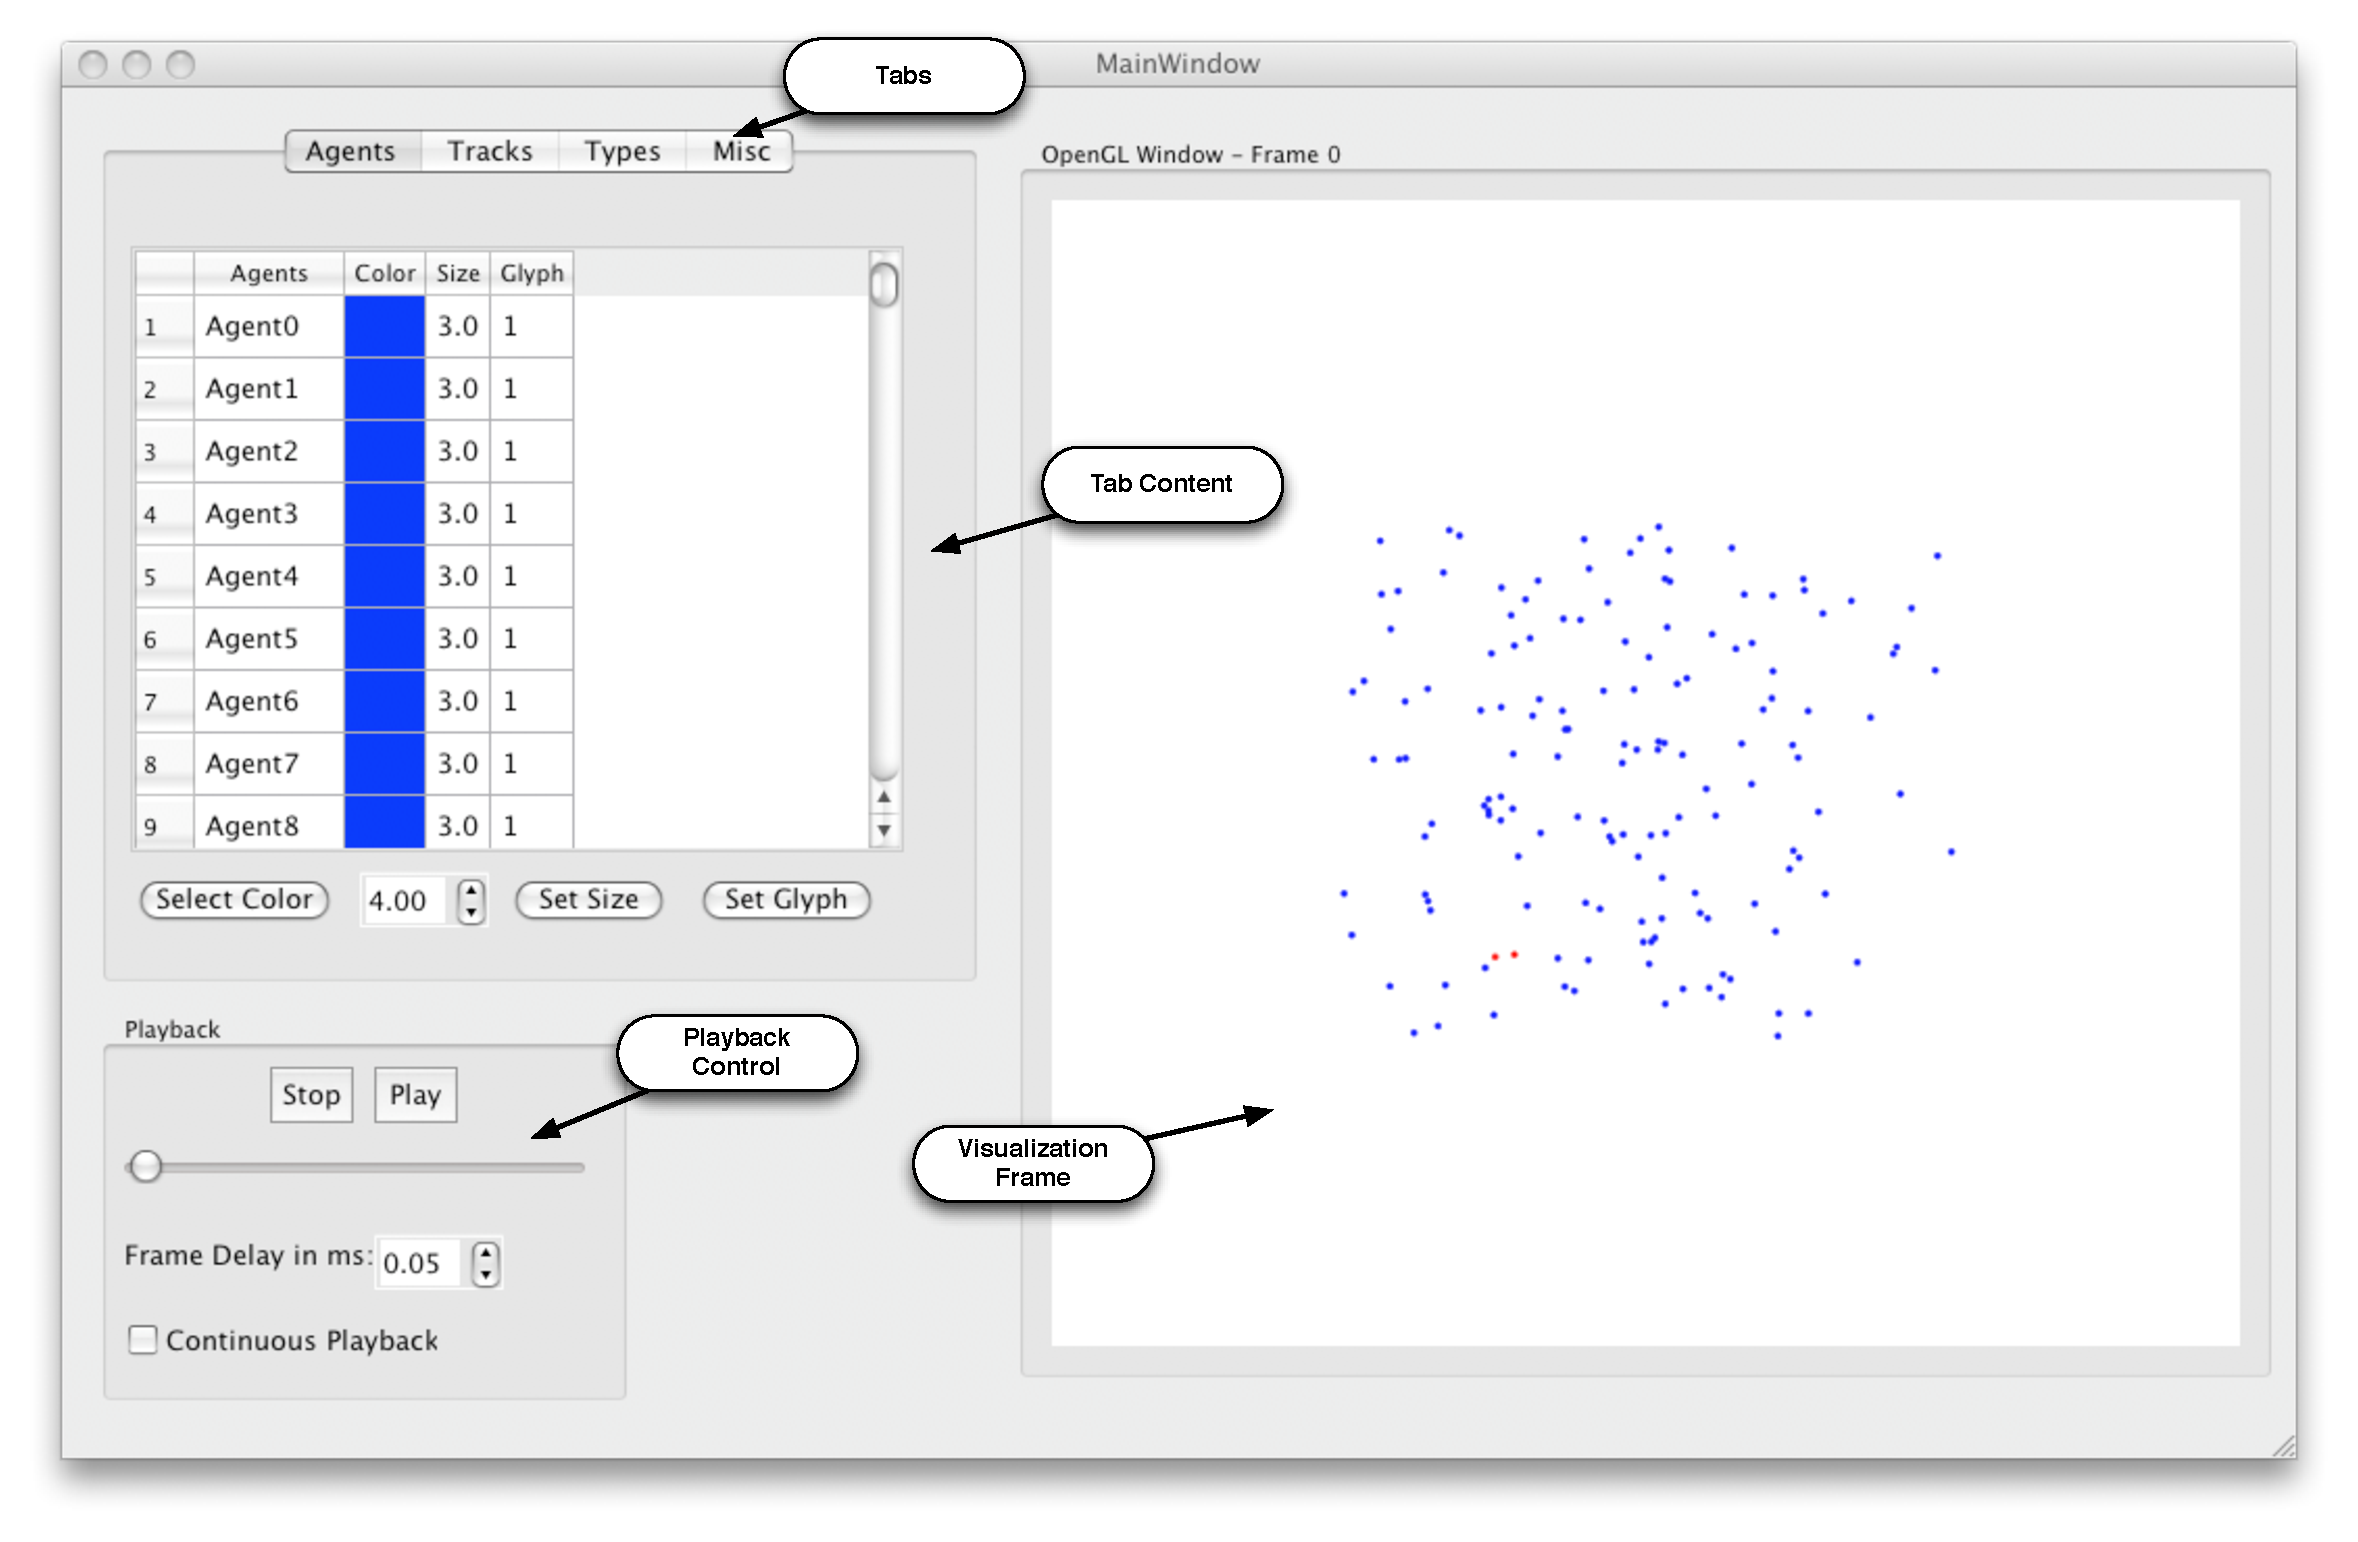
\includegraphics[scale=.45]{images/swarmvis-annotated.pdf}
\caption{The SwarmVis graphical user interface. 
The interface is split between the user controls (left) and the visualization (right).
There are tabs at the top left that give options for different visualizations in the tab content frame.
The playback frame, in the bottom left, works similar to a standard media player.
The visualization frame shows the swarm with all selected visualizations applied to it.
In this screenshot, the user has two agents colored red with all no other options enabled.
A file menu (not shown) allows for the loading of swarm data sets.}
\label{AnnotatedWindow}
\end{figure*}

\section{Approach}
The goal of SwarmVis is to facilitate, through visualization, the detailed analysis of emergent behavior that results from swarm systems.
We have implemented SawrmVis
with the following high-level application goals and requirements in mind:
\begin{itemize}
\item The toolkit shall visualize swarms using a series of still images (i.e. an animation)
embedded in an interactive user interface that has features such as pausing, slowing down and rewinding of frames.
\item Agent position, direction and velocity shall be conveyable through both still images and videos generated from the software.
\item The toolkit shall provide a variety of built-in visualization techniques that are useful in visualizing swarm systems.
\end{itemize}


SwarmVis is implemented in the C++ language and utilizes the Qt framework\cite{Qt:website} to build the graphical user interface.
The OpenGL library is used to render all visualizations.
The motivation of using Qt and OpenGL is to ensure SwarmVis' cross-platform compatibility.
The user interface is divided into a settings/options frame and visualization frame (see Figure \ref{AnnotatedWindow}).
The settings/options frame (left) contains the majority of the user interface,
whereas the visualizations frame (right) contains  the graphical display.
Any changes made to the visualization through the interface are applied to the current visualization in real-time.
The visualization frame can be rotated and zoomed by dragging and scrolling a mouse.
Lists and parameters are populated when a data set is loaded (more information about data sets is available in the appendix).

Still images can be created in SwarmVis by dumping the graphic currently shown in the visualization frame.
Videos can be constructed by having SwarmVis automatically dump every frame in the course of an animation.
These images can be compiled into a video by a third-party program that is used to make stop-motion
videos.\footnote{Boid flock and tetrahedron-forming swarm videos made by SwarmVis:\\
 http://maple.cs.umbc.edu/~don/projects/SAF/videos/\#tetra}

In the remainder of this section, we list the available visualizations in SwarmVis.
For each visualization, we discuss
(1) what they convey,
(2) how they are implemented,
(3) how they are enabled in the interface,
and (4) how their parameters can be adjusted.


\subsection{Visualizations}\label{visualizations}


\begin{figure}
\centering
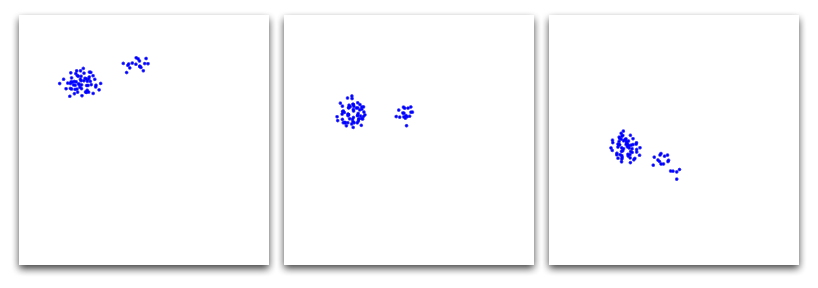
\includegraphics[scale=.282]{images/animation.png}
\caption{
Three captured frames from a three-dimensional flocking boids\cite{reynolds1987} animation.
The flocks' motion and structural changes are easily detectable when viewed in quick succession as frames in a video.}
\label{Animation}
\end{figure}

\subsubsection{Animation}

The playback control (as seen in  seen in Figure \ref{AnnotatedWindow})
gives the user the ability to specify what time step is being shown in visualization frame.
The inspiration for this control is any standard media player, such as QuickTime Player or Windows MediaPlayer.
The control provides the ability to stop, play, and manually move through frames with the slider.
In addition, the user can specify how fast the animation is played by adjusting the amount of delay between
frames (``Frame Delay" box).

Viewing a swarm over several time steps conveys a great deal of information.
It conveys direction, velocity, and structure by displaying how the swarm changes from time step to time step.
An example of this is shown in Figure \ref{Animation}, in which a swarm is shown to be
generally moving south while two sub-swarms begin to merge.
SwarmVis manages to make these animations incredibly smooth on a modern
computer,\footnote{2.2 GHz MacBook Pro running Mac OS X 10.5} even with a fast frame rate and hundreds of agents.
All of SwarmVis' applicable visualizations (i.e., color, size, trails, tracks) can be seen in fluid animation.








\begin{figure}
\centering
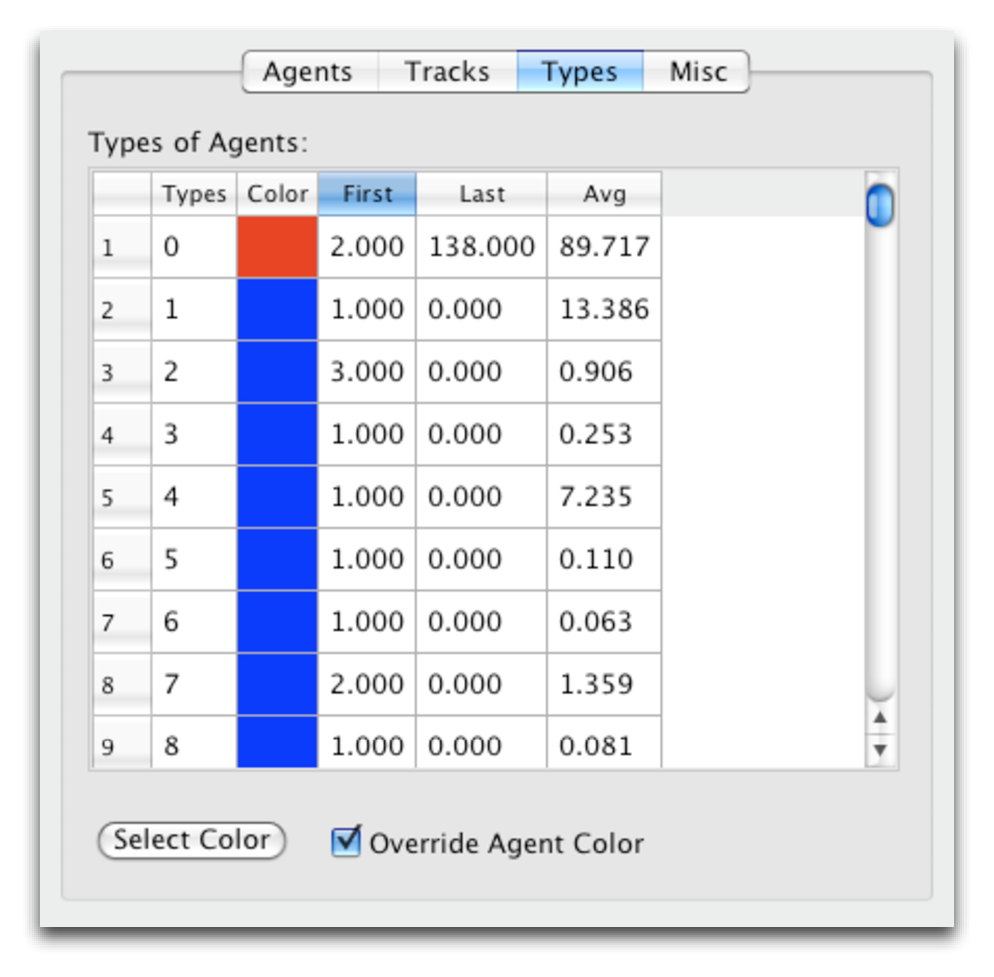
\includegraphics[scale=.5]{images/typestab.pdf}
\caption{
The Types tab shows the user which different subgroups exist in the swarm and allows the user to assign a specific
color to that group. Supplemental information helps the user
select the groups he wants: First (number of agents in that group in the first frame),
Last (number of agents in that group in the last frame), and Avg (average number of agents in that group during
the entire animation).}
\label{TypesTab}
\end{figure}

\begin{figure}
\centering
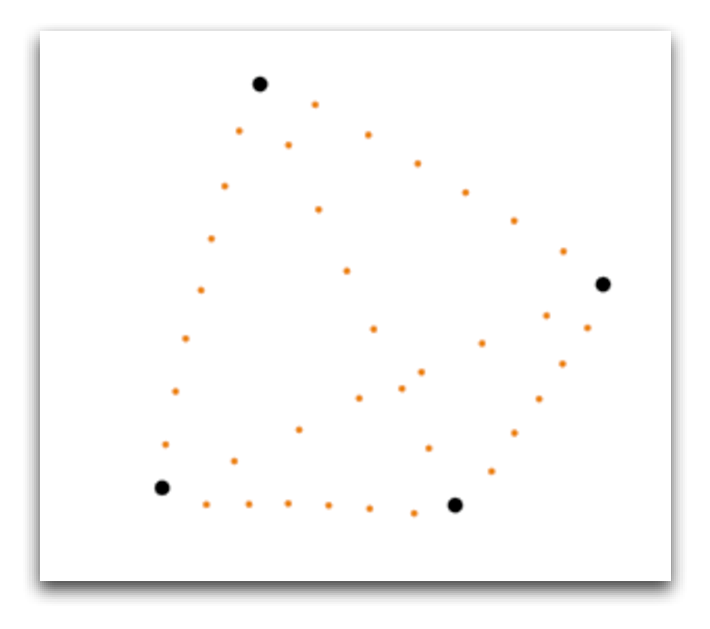
\includegraphics[scale=.4]{images/sizeandcolor.pdf}
\caption{
A captured frame from a swarm of tetrahedra-forming boids.
The corner agents have been given a larger size and a darker color than the edge agents.}
\label{SizeAndColor}
\end{figure}


\begin{figure}
\centering
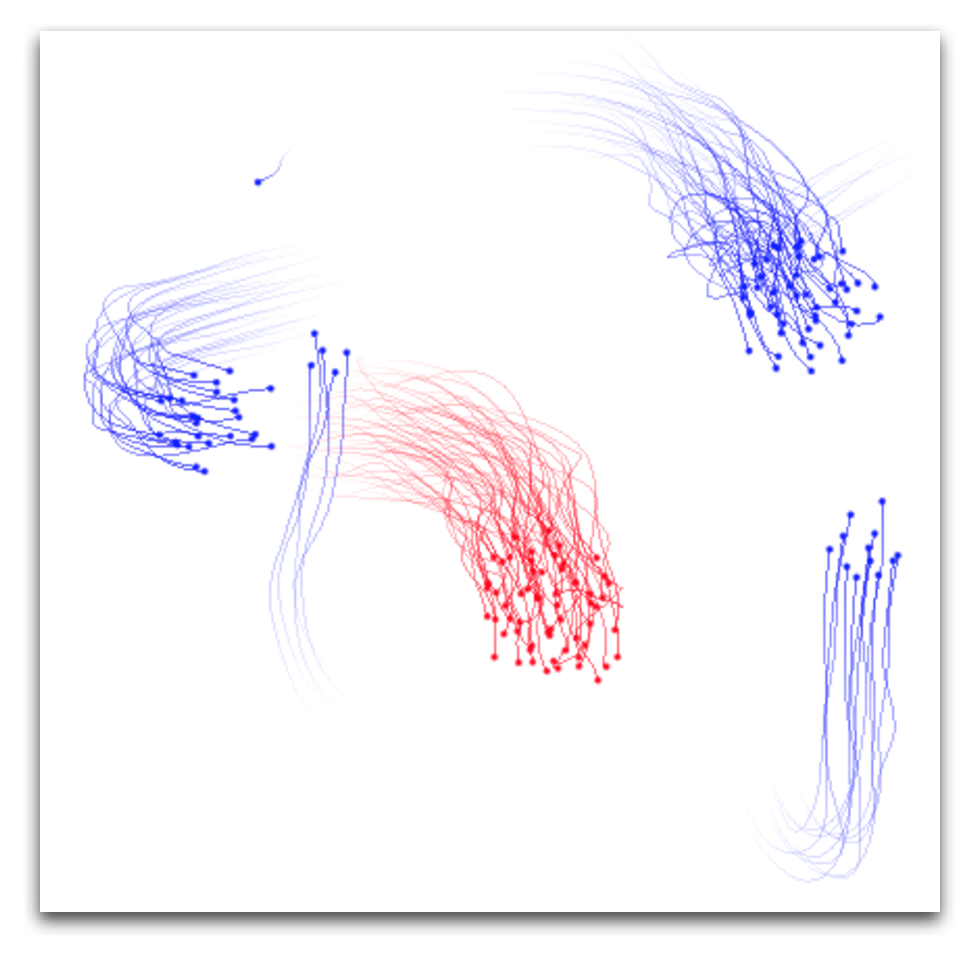
\includegraphics[scale=.45]{images/flockcolor.pdf}
\caption{
A captured frame from the three-dimensional flocking swarm shown in Figure \ref{Animation}.
The trails in this image are of length 35 time steps and agents of a particular chosen group are colored red.}
\label{FlockColor}
\end{figure}


\subsubsection{Color and Size}

SwarmVis allows for the effortless tracking of individual agents.
This can be done by selecting any number of agents of interest in the list of agents
(seen in the content frame of Figure \ref{AnnotatedWindow})
and changing their color or size with the button controls.
For example, in Figure \ref{SizeAndColor}, some agents have been made larger to emphasize their importance.

In addition, users can change the color of all agents that are members of a specific group in the \textit{Types} tab, as seen
in Figure \ref{TypesTab}.
This feature can be used in conjunction with varying sizes to emphasize particular agents.
For example, in the swarm shown in
Figure \ref{SizeAndColor}, we color the corners \textit{black} and the edges \textit{orange}.
Another example is shown in Figure \ref{FlockColor}, in which the largest flock of agents is colored \textit{red}.
The remaining agents are colored in \textit{blue} (default color).
Changing the color of the largest flock in the flocking domain is
particularly useful because it shows when two groups merge by changing the agents' colors as they collide.
Also, this feature is useful for creating figures for articles describing swarm research because
 the author can refer to specific agents as, for example, ``the large dark agents."





\begin{figure}
\centering
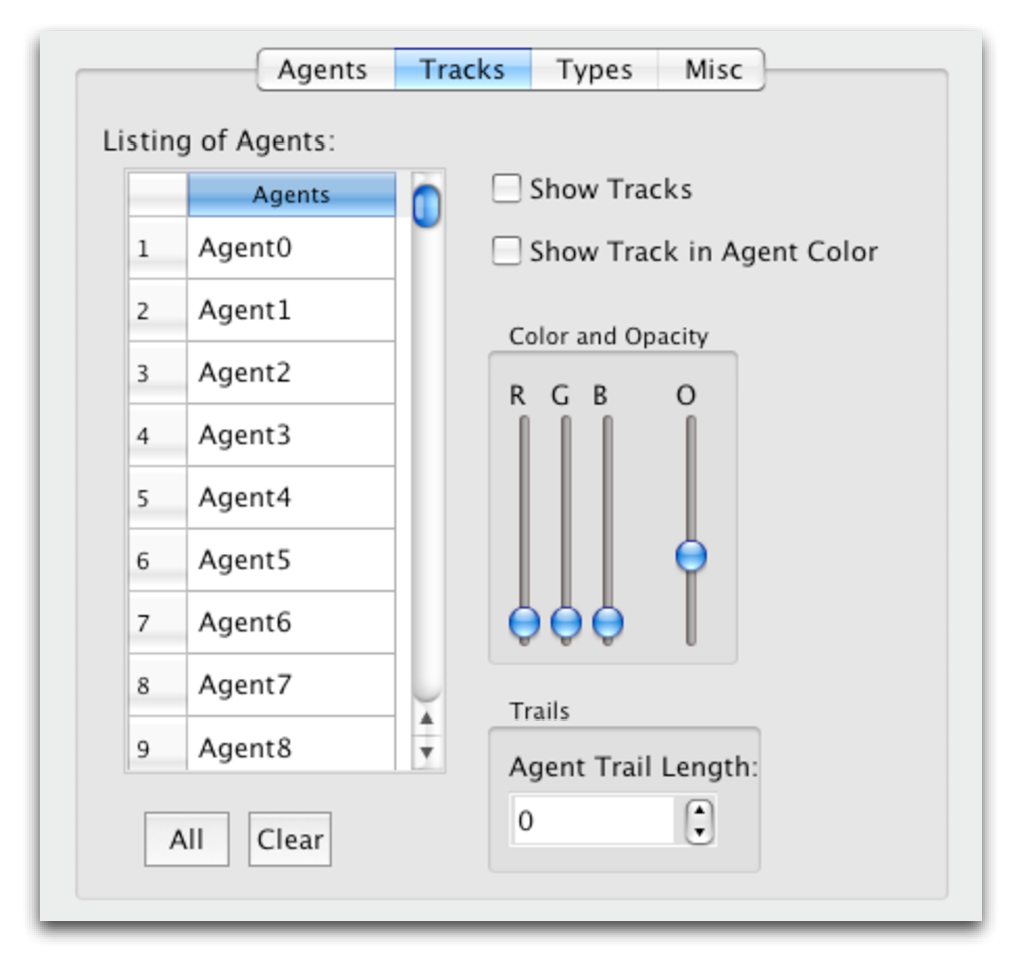
\includegraphics[scale=.5]{images/trackstab.pdf}
\caption{
The \textit{Tracks} tab allows users to add tracks and trails to agents. The length of the trails can be adjusted 
via the ``Agent Trail Length" box. }
\label{TracksTab}
\end{figure}

\begin{figure}
\centering
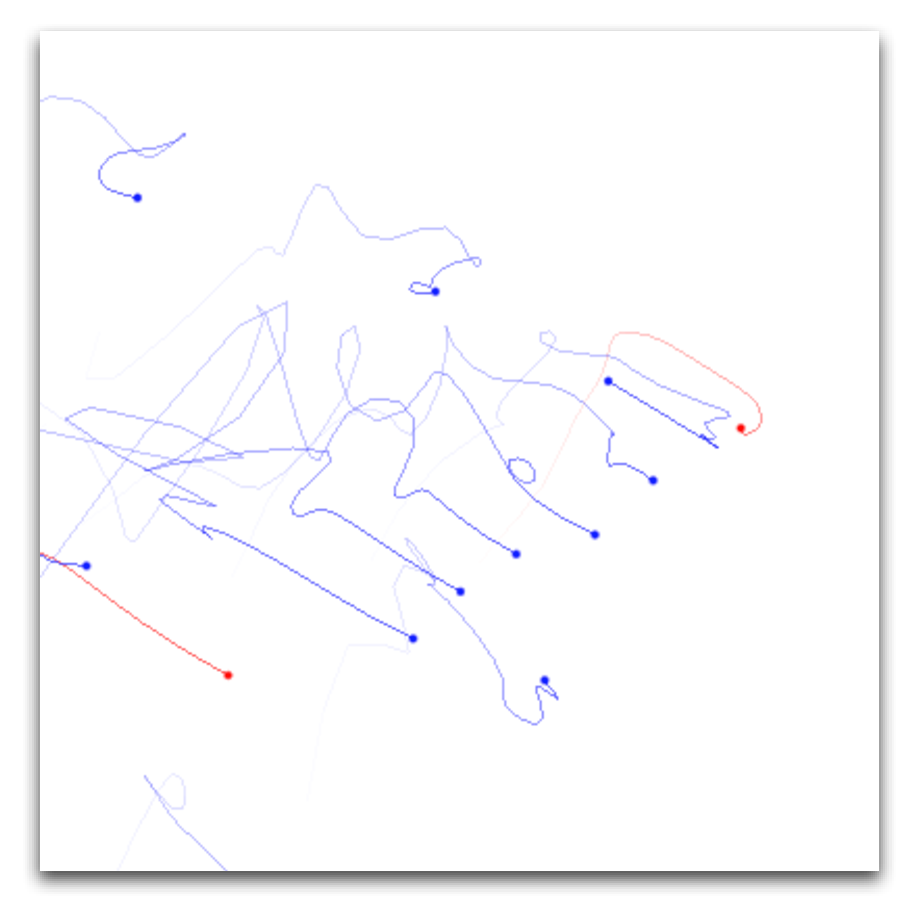
\includegraphics[scale=.5]{images/closeuptrails.pdf}
\caption{
A captured frame from a swarm of tetrahedra-forming boids shown in Figure \ref{SizeAndColor}.
Close up views of the swarm can convey much information about how agents interact with one another.
In this frame,  the right-most red corner agent swapped places with the rightmost edge agent.
Then, edge agents fill in the gap by moving to the right. The different times in which each adjustment happened
is shown by how long ago a ``notch" occurred in the trail.}
\label{CloseTrails}
\end{figure}

\subsubsection{Trails}

An agent trail is a set of line segments that represent the agent's previous $k$ positions, where $k$ is a number of time steps.
This is one of the most important features in SwarmVis because trails convey motion, previous positions, direction,
and change in structure.
The trails are created by connecting previous positions of the agents with
successive lines (i.e., linear interpolation) that are more opaque near the head of the agent and less so further back in time.
The length of trails can be adjusted in real-time via the ``Agent Trail Length" text box, shown in
Figure \ref{TracksTab}.

Trails can be used to view swarm behavior at an abstract level, such as tracking the motion of several boid
flocks at once, as seen in Figure \ref{FlockColor}.
However, one of the most powerful abilities of trails is to convey low-level behavioral information in swarms.
For example, in Figure \ref{CloseTrails}, we can see that the right-most corner agent (colored \textit{red})
swapped position with the right-most edge agent (colored \textit{blue}).
Then, all the agents in that edge shifted down to eliminate the newly formed gap.
The delay in the neighbors' reactions is shown by the ``notch" in the path happening
further back in time for the left agents, and more recently for the right agents.
This visualization feature makes qualitative analysis of agent behavior possible -- both at a low interaction level
and a high emergent level.







\begin{figure}
\centering
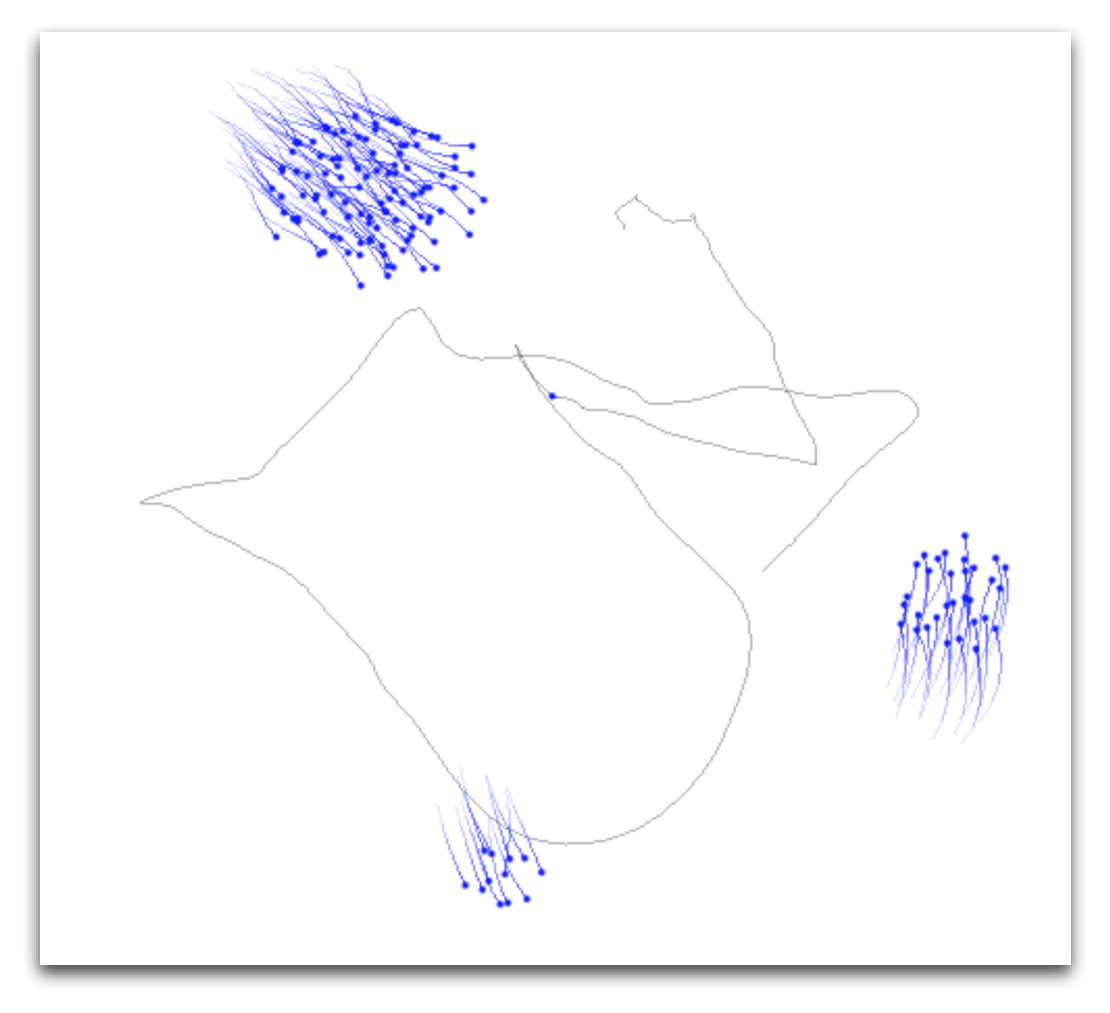
\includegraphics[scale=.4]{images/track.pdf}
\caption{
A captured frame from the three-dimensional flocking swarm shown in Figure \ref{Animation}.
The lonely agent (marked by being larger and darker) in the middle follows the traced path over its lifetime.
The track is colored based on velocity, showing that it moved rather slowly while being solitary (blue portion).
The agent then sped up after being picked up by a flock (red portion).
This event is inferred by the ``notch," as well as the change in color between the blue portion of the  path and the red portion of the path.
The structure of the line in three-dimensional space is more apparent while interactively rotating the visualization frame.}
\label{Track}
\end{figure}


\subsubsection{Tracks}

The tracks feature is very similar to the trails feature. Unlike trails, tracks show the position of an agent over the entire
lifetime of the system. At any given frame, the agent can be found at its respective position on the track.
A track of a single agent is shown in Figure \ref{Track}.
Several agents can be selected at once in the list of agents in the \textit{Tracks} tab (Figure \ref{TracksTab}) to
have all their trails shown at once.
When tracks are used in conjunction with trails, the trails are overlaid on top of the tracks so that
both trail and track information is conveyed.





\begin{figure}
\centering
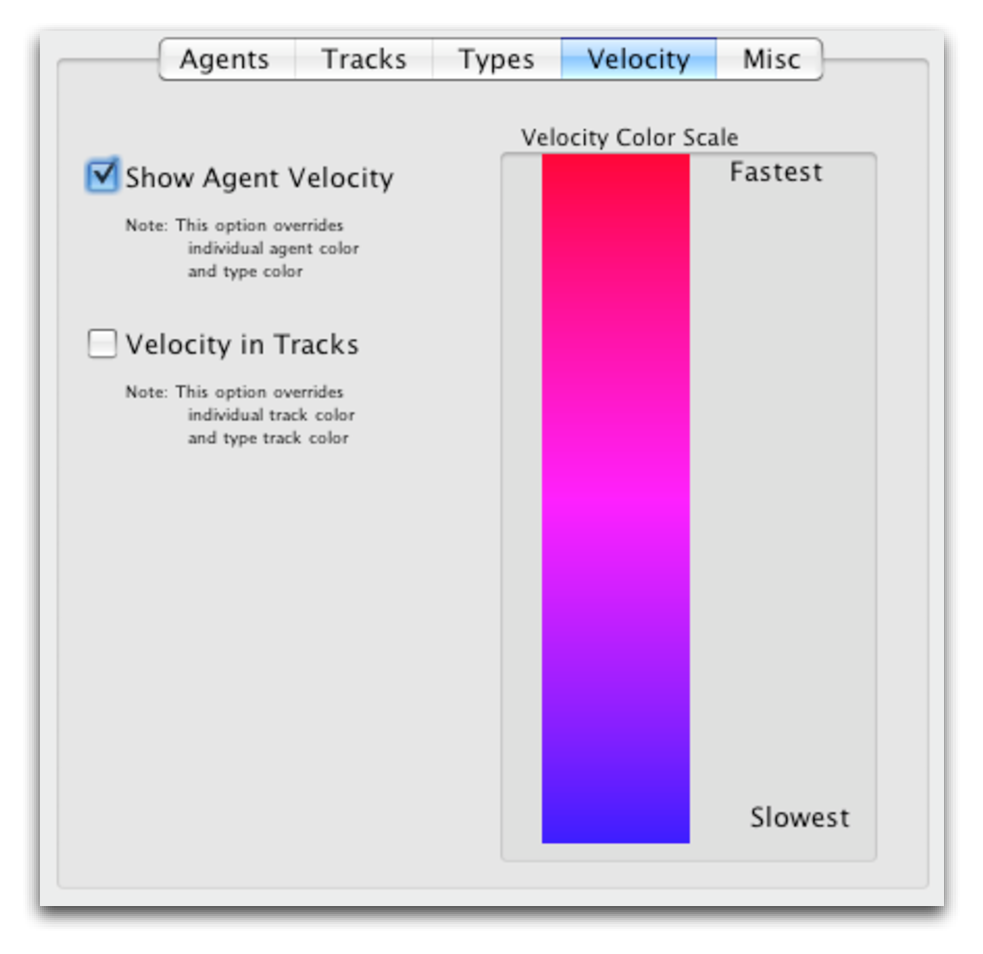
\includegraphics[scale=.5]{images/velocitytab.pdf}
\caption{
The \textit{Velocity} tab allows users to map agents' velocities to a color, shown in the gradient on the right.
The ``Show Agent Velocity" option will color the agent and its entire trail (if enabled) more red if the agent is moving relatively fast,
or more blue if the agent is moving relatively slow (seen in the right image of Figure \ref{Velocity}).
The ``Velocity in Tracks" option visualizes velocity on the track of an agent.
The track's color matches the speed of its agent at that time step (seen in the left image of Figure \ref{Velocity}).}
\label{VelocityTab}
\end{figure}

\begin{figure*}
\centering
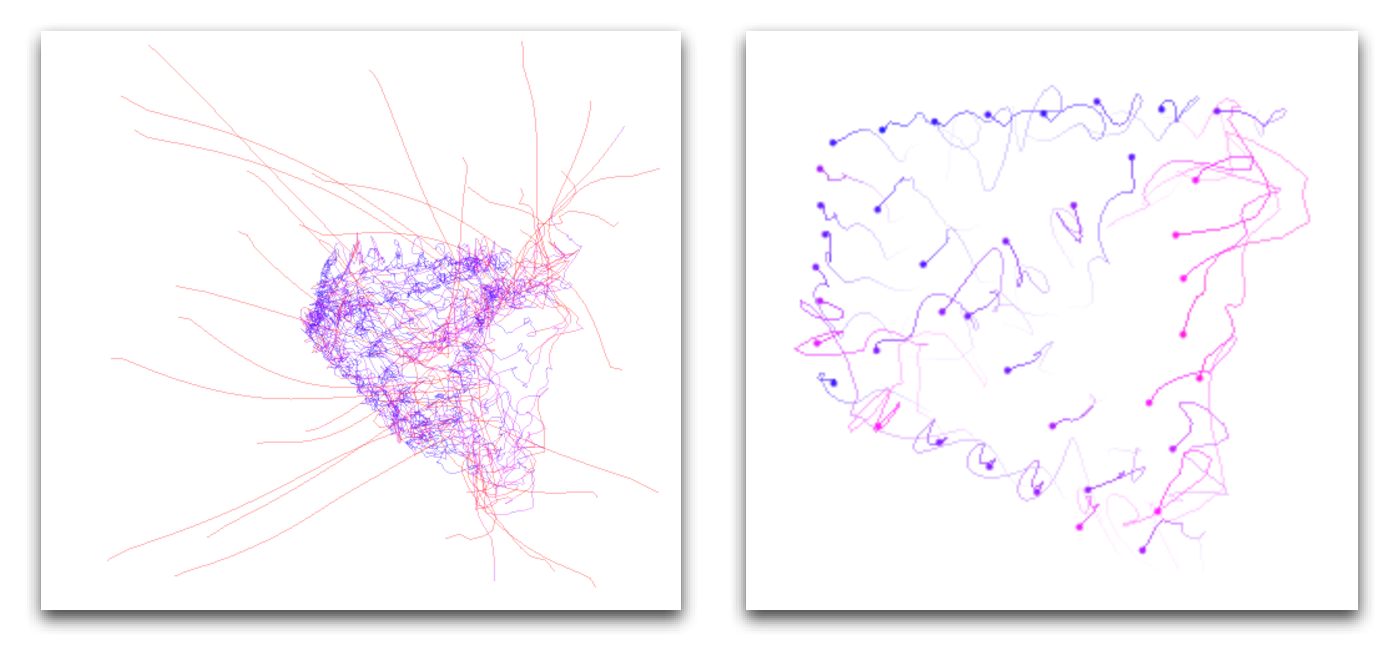
\includegraphics[scale=.667]{images/velocity.pdf}
\caption{
A captured frame from a swarm of tetrahedra-forming boids shown in Figure \ref{SizeAndColor}.
On the left, all agent tracks are displayed, showing that agents move faster (the color red) at the beginning.
Once the agents organize into the tetrahedron they slow down (the color blue).
On the right, the trails and the agents themselves are colored according to their instantaneous velocity.
From this captured frame, it is obvious that the right edge is experiencing movement while the rest of the
shape is calm. }
\label{Velocity}
\end{figure*}

\subsubsection{Velocity Color}

The velocity feature is useful for displaying the instantaneous or historical velocity of agents.
This visualization can be applied in two different ways:
(1) color each agent and its corresponding trail according to the agent's current instantaneous velocity and/or
(2) color the agent tracks based on the velocity at each respective time step.
SwarmVis uses the distance traveled in one time step to determine the velocity of an agent, then calculates the 
intended color from a color gradient.
The default color gradient is determined by assigning the highest and lowest velocities found in a data set to the colors \textit{red} and \textit{blue}, respectively (see Figure \ref{VelocityTab}).

Assigning agent color to instantaneous velocity conveys the changes in velocity while viewing the swarm as an animation or a still image.
Agents that are moving faster are colored differently than agents that are moving slower.
An example of this is shown in Figure \ref{Velocity} (right).
Coloring the entire trail the instantaneous velocity (opposed to its default color) makes the color and velocity change more obvious,
thereby drawing the user's attention.

Coloring tracks based on the velocity is a powerful feature that displays how an agent's or an entire swarm's
velocity changes over the course of the system.
Every line segment in the track is colored based on its length. The Euclidean distance measure is used to calculate distances in space: the longer the segment, the more distance an agent traveled in one time step,
and thus the faster the agent was moving.
A single agent's track is pictured in Figure \ref{Track}, in which we see how the velocity of this particular agent changes over the course of its lifetime.
In Figure \ref{Velocity} (left), every agent has its track shown.
From this image, we can determine that the movement is very fast and chaotic in the initial phases, but calms to a slower speed once the agents have organized into the shape.

\section{Results: Analysis of the Tetrahedron-Forming Swarm}

%Throughout the course of this document, we have discussed the motivation behind the visualizations in SwarmVis by
%displaying images from two data sets: a boid flock and a tetrahedron-forming swarm.
To demonstrate that SwarmVis is effective,
we provide a cohesive and comprehensive walk-through of how a user would
analyze the tetrahedron-forming swarm. First, we provide domain background information.
Second, we analyze the images and animations provided by SwarmVis and show how information not evident directly from the data sets is conveyed.

\subsection{Background}

The shape is formed by agents adhering to the following procedure.
First, four corners are selected by the swarm via a simple election algorithm.
Then, the agents persistently execute the following rules:
\begin{itemize}
	\item If a corner, be attracted slightly to the three other corners.
	\item If not a corner, be attracted to the two closest corners with great, but equal, strength.
	That is, the output force vector of this rule is the sum of two vectors with some constant and equal magnitude.
	Note the forces cancel each other out when an agent is on the line formed by its two closest corners,.
	\item Move away from agents that get too close.
\end{itemize}

\begin{figure*}[ht]
\centering
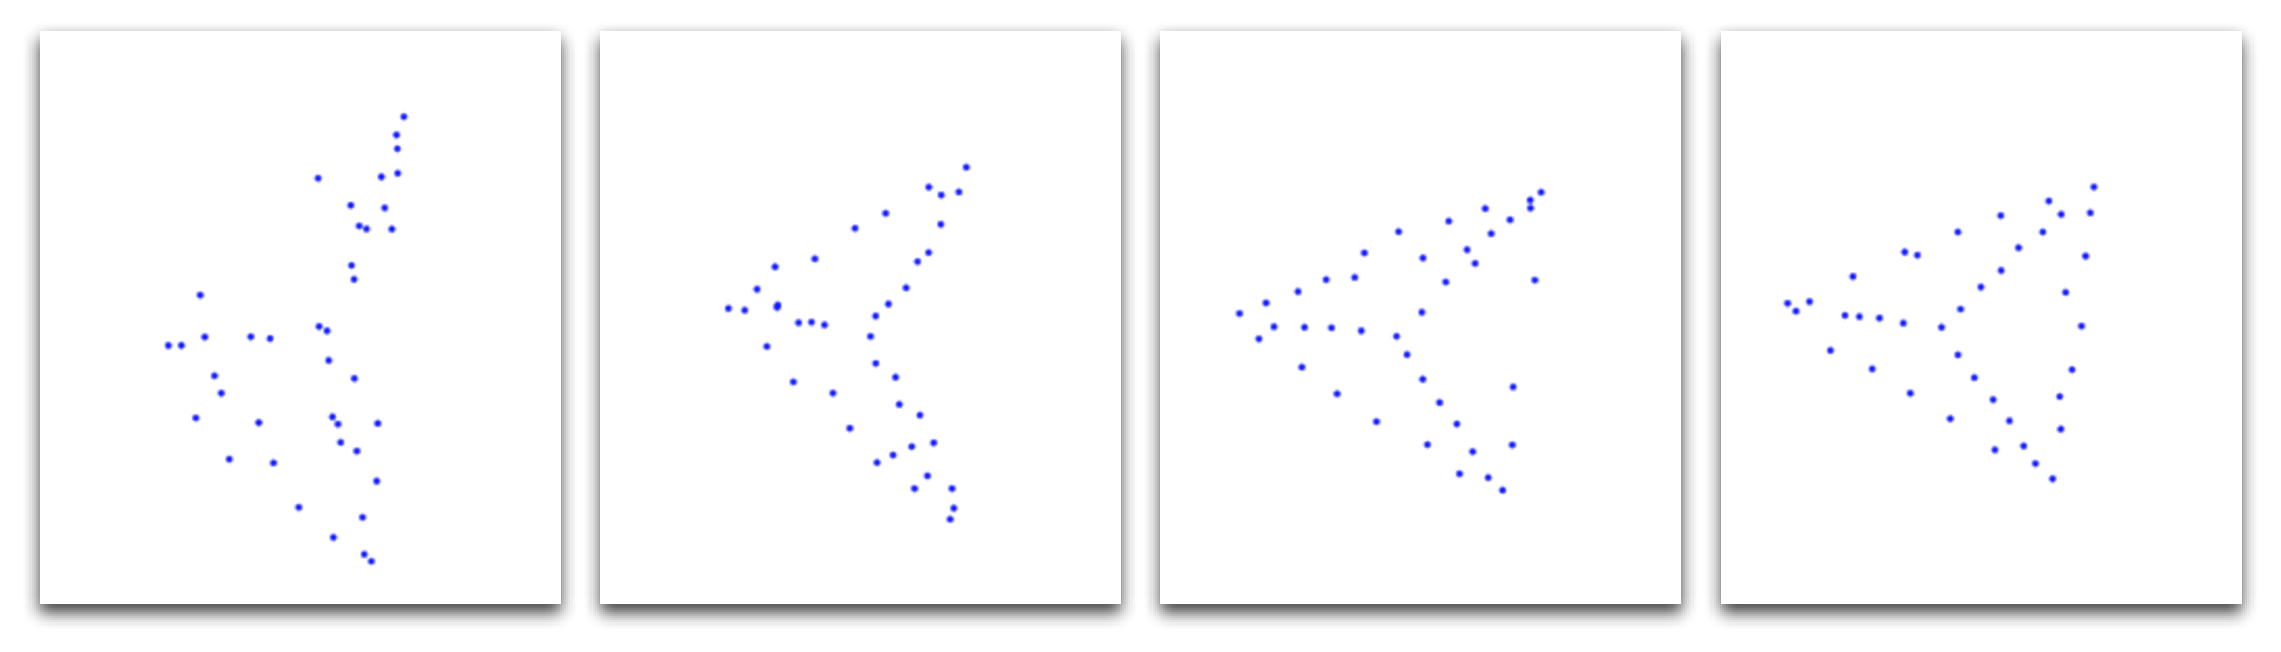
\includegraphics[scale=.3]{images/tetraclosing.pdf}
\caption{
The tetrahedron-forming swarm uses an emergent strategy to form its last (sixth) edge.
The swarm initially forms two triangles with a shared edge (total of five edges), then
closes in on itself to form the last edge. This is easily noticed while watching the swarm in animation.}
\label{TetraClosing}
\end{figure*}

The end result of these rules are somewhat obvious: the agents self-organize into a tetrahedron.
However, many of the fine-grained details of this behavior are not clear.
For example, some questions one may want to ask about this system are: 
\begin{itemize}
\item Will the shape formed be equilateral?
\item How stable is the shape once it is formed? Does it reach an equilibrium and stop moving? If not, what is changing?
\item How do agents react to movement in the tetrahedron?
\item How fast do agents create a shape that is a discernible tetrahedron?
\item Are there any interesting ``emergent strategies" that this swarm uses?
\end{itemize}
These and other questions are not easily answerable by studying the rules or the raw position data.
The purpose of SwarmVis is to provide users with the power to answer these questions,
as well as to identify emergent behaviors not previously expected to exist.

The particular tetrahedron-forming swarm data set we will be analyzing in this section has forty agents
and is comprised of 333 individual frames of agent coordinates.



\subsection{SwarmVis Analysis}
SwarmVis has several tools available to analyze swarms and to create informative visualizations.
To demonstrate the results of our work, we provide examples of how the tetrahedron-forming swarm can be analyzed.
Due to the nature of these complex systems, there are always new behaviors waiting to be found.
SwarmVis enables the user to discover these points of interest, which otherwise would be hard to identify.
\footnote{The tetrahedron
data set is available from the SwarmVis project website: http://swarm-vis.googlecode.com/files/tetrahedra\_boids.zip}




\subsubsection{Animation}

Several interesting observations can be made by viewing the swarm with an animated series of plotted points.
From an animation of the tetrahedron-forming swarm,
we immediately determine that the swarm is initially spread thin without any organization.
Then, agents move towards the center and follow an emergent strategy (i.e., not explicitly part of the agent rules)
to form the sixth edge of the tetrahedra: Two triangles are formed with a shared edge (five edges) then two corners collapse in on themselves, forming the sixth edge. Agents executing this strategy are shown in Figure \ref{TetraClosing}.
After this, we can see the swarm moving towards the center of the screen in a stable manner.
Then, surprisingly, agents start bouncing back and forth from edge to edge, not permitting the tetrahedron to
reach an equilibrium. Other than these obvious facts, not much more information can easily be inferred by watching this simple animation.

Our first step in making more useful visualizations is to color the corners differently than the rest of the agents so that
they are easier to track. We see in the \textit{Types} tab (Figure \ref{TypesTab}) that there are two groups, labeled
``corner" and ``edge" (agents are explicitly labeled in the data set). Although the labels are intuitive, we can also infer that the second group in the list contains the corner agents because it has an average of 3.988 member agents over the lifespan of the swarm.
Since a tetrahedron has four corners, it is safe to assume that this group contains the corners we wish to color.
This feature is important in this domain because the corner agents follow different rules than the edge agents.
Therefore, segregating them will make it easier to understand how the swarm functions.
At this point of the walk-through, our visualization shows a tetrahedra similar to that in Figure \ref{SizeAndColor}.

%The best way to share animations is to create a video with SwarmVis.
%Videos would be appropriate for sharing information conveyed by an animation online or in presentations.

\begin{figure}
\centering
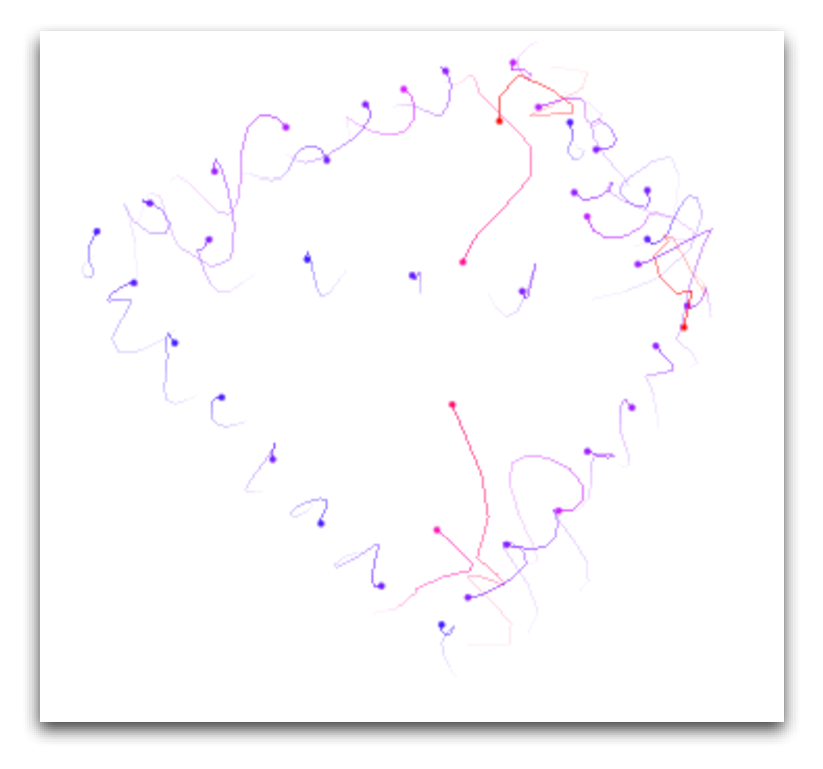
\includegraphics[scale=.5]{images/tetrastrategy.pdf}
\caption{
The tetrahedron-forming swarm creating its sixth edge with velocity-colored trails enabled.
}
\label{TetraStrategy}
\end{figure}

\subsubsection{Trails}

Previously, in Figures \ref{CloseTrails} and \ref{Velocity}, we described how trails can convey important information.
We now add another example of how powerful of a tool agent trails are in creating compelling still images.
Velocity-colored trails can be used to explore how the tetrahedra-forming swarm is completing the sixth edge of the shape.
The trails show where the agents are coming from and where they are going.
With the addition of the velocity coloring we can easily see which agents are shifting significantly.
By zooming in close to the sixth edge as it closes and taking a still image at the appropriate time (which we found
by moving our slider slowly), we obtain the image shown in Figure \ref{TetraStrategy}.
From this image, we can extrapolate that the edge agents closest to the corners are the ones that form the new edge.
These agents move very quickly, represented by their red coloration.
Meanwhile, agents from the edges where these ``quick'' agents were located initially, shift downwards to fill in the gap.
These gap filling agents are colored purple due to their slightly slower movements.
At this point, we feel we have a detailed understanding of how the last edge is formed through this emergent strategy.
Without trails, this phenomena could not have been demonstrated in a single image (e.g., see Figure \ref{TetraClosing})
or from raw data.



\begin{figure*}[ht]
\centering
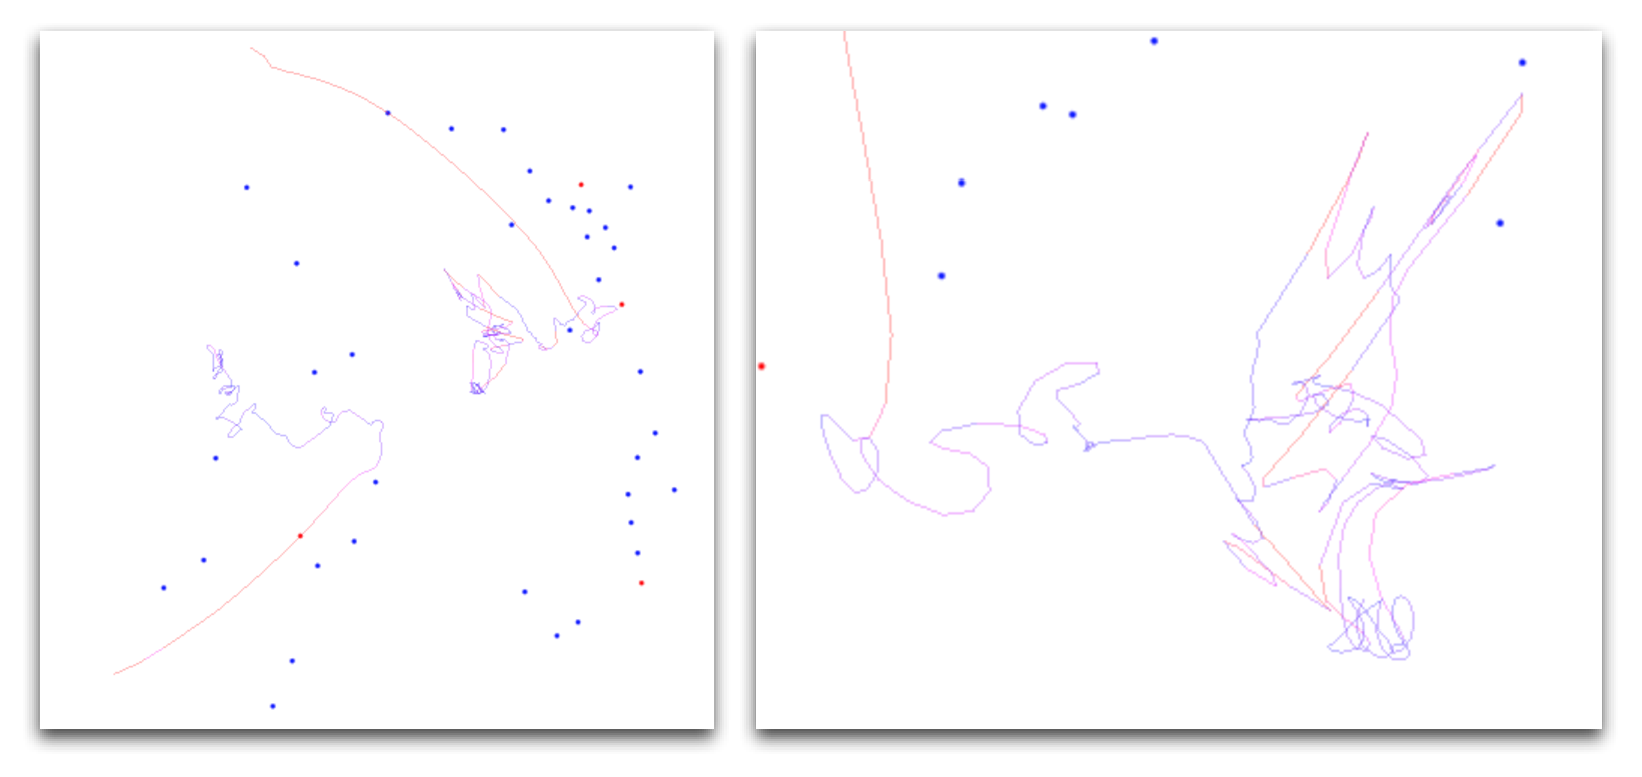
\includegraphics[scale=.5]{images/cornervsedge.pdf}
\caption{
(Left) A comparison of a corner's track and an edge agent's track.
The two can be contrasted by analyzing the color and structure of the tracks.
The corner agent gets into position and remains relatively calm for the remainder of the time.
(Right) Meanwhile, the same edge agent goes through several high-speed moments and never reaches a steady state.
}
\label{CornerAndEdge}
\end{figure*}

\subsubsection{Tracks}
In Figure \ref{Velocity}, we showed that velocity colored tracks can be used to get a high-level view of the swarm behavior.
Colored tracks can also be used to infer information about an individual agents' behavior.
To gain insight into agent behavior, we cycle through several agents listed in the \textit{Tracks} tab.
Very quickly, we realize that there is a significant difference between the behavior of a corner agent and a typical edge agent.
A visual comparison of the two types of agents is given in Figure \ref{CornerAndEdge}.
From the images shown in this figure, we see that the life of an edge agent is far more chaotic than that of a corner agent.
A corner agent barely changes position after reaching its desired location.
On the contrary, the movements of edge agents are highly variable in terms of both position and velocity.
In some situations, selecting agents that end up as neighbors can convey information about how they affect one another.





\section{Future Work}
There are a several user interface changes that could improve overall usability.
In the future, we would like to simplify the agent selection process in the interface as well as the graphical display.
To facilitate this functionality, we hope to implement text labels adjacent to each agent in the visualization window.
Furthermore, the ability to click agents in the visualization window would allow for greater interactivity and easier modification of agent-level colors and effects.

Currently, each visualization effect is controlled by a separate procedure.
In effect, separate agent lists are kept in the \textit{Agents} tab, the \textit{Tracks} tab and the \textit{Types} tab.
Therefore, any modifications made to a particular visualization (e.g., changing the color of an agent) is not reflected in the other lists.
Having an interactive global agent list that displays all necessary information would enable users to modify
the colors and effects on groups of agents more effectively. 

Additionally, we plan on implementing the ability to change the dot representation of the agent to better display direction.
Currently, direction is inferred by the direction of the trails.
However, direction is not always apparent,
especially when (1) trails excessively overlap or (2) agents change direction quickly and unexpectedly.
Previous work has represented agents as  pyramids\cite{spector2005ecb}  and ellipsoids\cite{10.1109/TVCG.2005.87}.
These are superior to dots since they explicitly show the direction of an agent.

To further increase the amount of information conveyed in still images,
we hope to develop a sufficient technique for displaying the depth of
agents, trails and tracks since this information is not explicitly visualized.
To our knowledge, the literature has not specifically dealt with this problem, prompting further investigation.

Finally, we plan on allowing SwarmVis to be more extendable by using a plug-in framework.
Any new visualization effects that are added to SwarmVis currently are hard coded into the main source code. This practice is not intuitive to a naive user who wishes to add his or her own visualizations.
Plug-ins could be implemented as simple programs that take the agent data as input and return
visualization primitives to be rendered on the screen.



\section{Conclusion}
We have demonstrated that SwarmVis is a powerful and dynamic tool.
It is a complete application that has accomplished all the original goals that we set out to achieve.
SwarmVis is able to create animations and still images that convey agent position, agent direction and agent velocity.
It can also help with the identification of many emergent properties of swarms, such as structure.
We believe that the set of visualizations provided makes this tool dynamic and applicable to many domains.

Our work simplifies the task of detailed analysis of emergent behavior and
enables swarm intelligence researchers to come to new conclusions previously not apparent.


\bibliographystyle{IEEE}
\bibliography{cmsc636-swarmvis}
\vspace{50pt}


%\pagebreak


\section{Appendix: User Guide}

\subsection{Compiling and Running}
SwarmVis is a cross-platform tool
and is intended to run on Unix-like systems, such as Mac OS X and GNU/Linux, as well as Microsoft Windows.
The source code is available at:\begin{quote}\texttt{http://code.google.com/p/swarm-vis/}\end{quote}
The following programs are required to compile SwarmVis from source:
\begin{itemize}
\item Qt 4.2
\item gcc/g++ 4.2.2
\item make
\end{itemize}
Note that some libraries from Qt4.2 may be needed to run the SwarmVis binary.
We have tested SwarmVis on Mac OSX 10.5 and openSUSE Linux 11.

Run \texttt{qmake}, and then \texttt{make}, both in the root directory, to compile SwarmVis.
A binary will be created in the \texttt{bin/} directory. Execute this binary to run SwarmVis.

\subsection{Data File Format}
SwarmVis requires a specific format for data sets that are to be loaded. The agents' position data is segmented into
separate files that each represent a single time step. These files contain space-delimited data, with
each row representing an agent. For example, a swarm system with 100 agents depicted over 500 time steps
will have 500 files in a folder, each with 100 lines of text.

Each row entry in a file must follow a specific format. The first two or three  columns (depending on dimensionality) are the
position data $(X, Y)$ or $(X, Y, Z)$, respectively. The last column is reserved for the group label, which may be used to pass
group membership data to SwarmVis.
For example, a well-formed entry that conveys a three-dimensional position with group information could be:
\begin{quote}
\texttt{10.15 5.24 84.85 Corner}
\end{quote}
The order of the listing of agents in each file must be consistent.
That is, the $k^{th}$ entry in one file and the $k^{th}$ entry in another file must represent the same agent.

A plain-text information file containing important meta-data must accompany the frame files in the same directory.
The following variables must be defined (i.e., \texttt{VARNAME = VALUE}) in this file in order for the data to be loaded appropriately:
\begin{itemize}
\item \texttt{DIMENSIONS} (\texttt{2} or \texttt{3})
\item \texttt{AGENTS} (the number of agents)
\item \texttt{FRAMES} (the number frames/time steps)
\item \texttt{RANGEX} (the maximum X value)
\item \texttt{RANGEY} (the maximum Y value)
\item \texttt{RANGEZ} (the maximum Z value)
\item \texttt{AGENTTYPES} (\texttt{1} to track agent types, \texttt{0} if not)
\end{itemize}
At the bottom of this file, the keyword \texttt{FILES} must appear, followed by a list of frame files, in ascending
temporal order.
The number of files listed here must equal the number specified by the \texttt{FRAMES} variable.
Also, the number of lines in every file must match the number specified by the \texttt{AGENTS} variable.
To load a data set in the SwarmVis application, navigate to ``Load Data" and select the info file.

A sample info file for a 150 agent three-dimensional swarm over the course of 446 frames:


\begin{verbatim}
     DIMENSIONS = 3
     AGENTS = 150
     FRAMES = 446
     RANGEX = 600
     RANGEY = 600
     RANGEZ = 600
     AGENTTYPES = 1
     FILES
     frame000001.txt
     frame000002.txt
     frame000003.txt
     frame000004.txt
     frame000005.txt
     frame000006.txt
     ...
     frame000442.txt
     frame000443.txt
     frame000444.txt
     frame000445.txt
     frame000446.txt
\end{verbatim}
\end{document}


